\documentclass[12pt]{article}

\usepackage{amsmath,amsfonts,amsthm,amssymb}
\usepackage{color}
\usepackage{graphicx}
\usepackage{wrapfig}
\usepackage{epsfig}
%\usepackage{subfigure}
\usepackage{times}
\usepackage{xspace}
\usepackage{url}
\usepackage{pdfpages}
\usepackage{array}
\usepackage{subfig}
\usepackage{multirow}
\usepackage{dblfloatfix} 

\setlength{\topmargin}{0.0in}     % top of paper to head (less one inch)
\setlength{\headheight}{0in}      % height of the head
\setlength{\headsep}{0in}         % head to the top of the body
\setlength{\textheight}{9.0in}    % height of the body
\setlength{\oddsidemargin}{-.25in} % left edge of paper to body (less one inch)
\setlength{\evensidemargin}{0mm}  % ditto, even pages
\setlength{\textwidth}{7.0in}     % width of body
\setlength{\topskip}{0in}         % top of body to bottom of first line of text
\setlength{\parindent}{1pc}       

\begin{document}
\thispagestyle{empty}
%%%%%%%%%%%%%%%%%%%%%%%%%%%%%%%%%%%%%%%%%%%%%%%%%%%%%%%%%%%%%%%%%%%%%%%%%%%%%%%%%%%%%%%%
% Project Summary
%%%%%%%%%%%%%%%%%%%%%%%%%%%%%%%%%%%%%%%%%%%%%%%%%%%%%%%%%%%%%%%%%%%%%%%%%%%%%%%%%%%%%%%%
\begin{center}
{\Large\bf Project Update \#1}
\vspace{3mm}
\\Caitlin Ross, Noah Wolfe
\\4/14/2016
\\*[3mm]
\end{center}

\section{Data Collection}
So far, we have spent the majority of our time generating and formatting our ever-increasing database consisting of Slim Fly and Dragonfly network simulation performance results. We have decided to make use of multiple hardware systems we have available including RPI's IBM Blue Gene/Q supercomputer and a smaller 64-core AMD workstation. Each simulation collects the discrete event simulation performance metrics such as rollbacks and remote events throughout the simulated time. Right now we are waiting on 720 simulation executions to complete and are expecting the simulations to take over 30 hours to execute and to generate multiple GBs of data.

\section{Unexpected Challenges}
In our ambitious attempt at fully understanding the difference between the Dragonfly and Slim fly network simulations, we are performing around 720 executions with different simulation parameters. This large number of runs provides us another higher-level data selection layer that we hadn't initially taken into account. We currently don't have a visualization that allows the user to interactively select subsets of runs to display their simulation results. Our current implementation would require the user to input each run separately to be analyzed on it's own.

\section{Changes}
In response to the unexpected challenge discussed in the previous section, we have decided to generate another parallel coordinates graph to the the top of the visualization layout. This parallel coordinates graph will present the high-level results for all simulation runs and allow the user to select one run or a collection of runs. After selection, the simulation results, network congestion, etc. will be displayed in the original visualizations. In the case that the user selects more than one run, then the results will be averaged for all selected runs. 

%\section{User Interface}
%\begin{figure*}[t]
%\centering
%   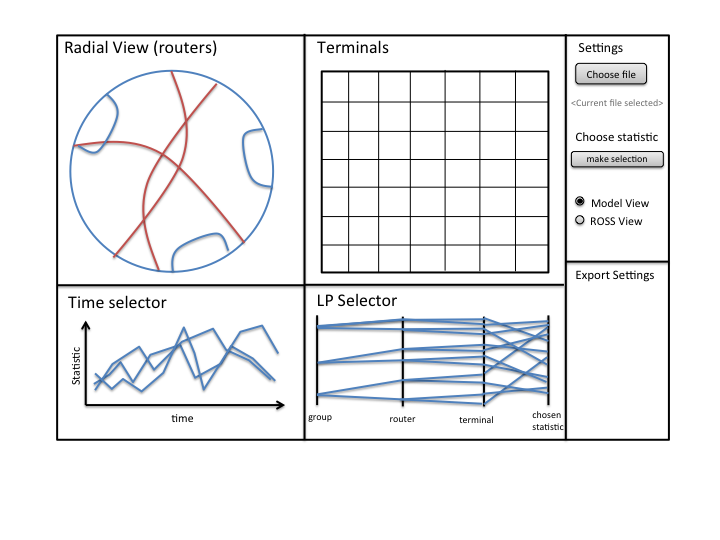
\includegraphics[width=6.5in, clip=true, trim=0 1in 0 0]{../figures/gui-diagram/Slide1.png}
%\caption{Model View}
%\label{model-view}
%\end{figure*}



%\end{document}  % This is where a 'short' article might terminate

%ACKNOWLEDGMENTS are optional
%\section{Acknowledgments}

%
% The following two commands are all you need in the
% initial runs of your .tex file to
% produce the bibliography for the citations in your paper.

% You must have a proper ".bib" file
%  and remember to run:
% latex bibtex latex latex
% to resolve all references
%
% ACM needs 'a single self-contained file'!
%
%APPENDICES are optional
%\balancecolumns


%\balancecolumns % GM June 2007
% That's all folks!
\end{document}
